%!TEX root = ../bdr.tex

\acode{08-02}%
\bcode{БКР}%
\ccode{000}%
\dcode{13}%
\ecode{000}
\fcode{Е3}
\partdes{Схема електрична принципова}%


\begin{drawing}
\chapter[(Довідковий) Приклад додатку у форматі кресленика довга назва для перевірки перенесення]{}
\label{apdx:ozpsch}
% \begin{picture}(0,0)
%   \put(-105,-740.6){\frame{\hbox{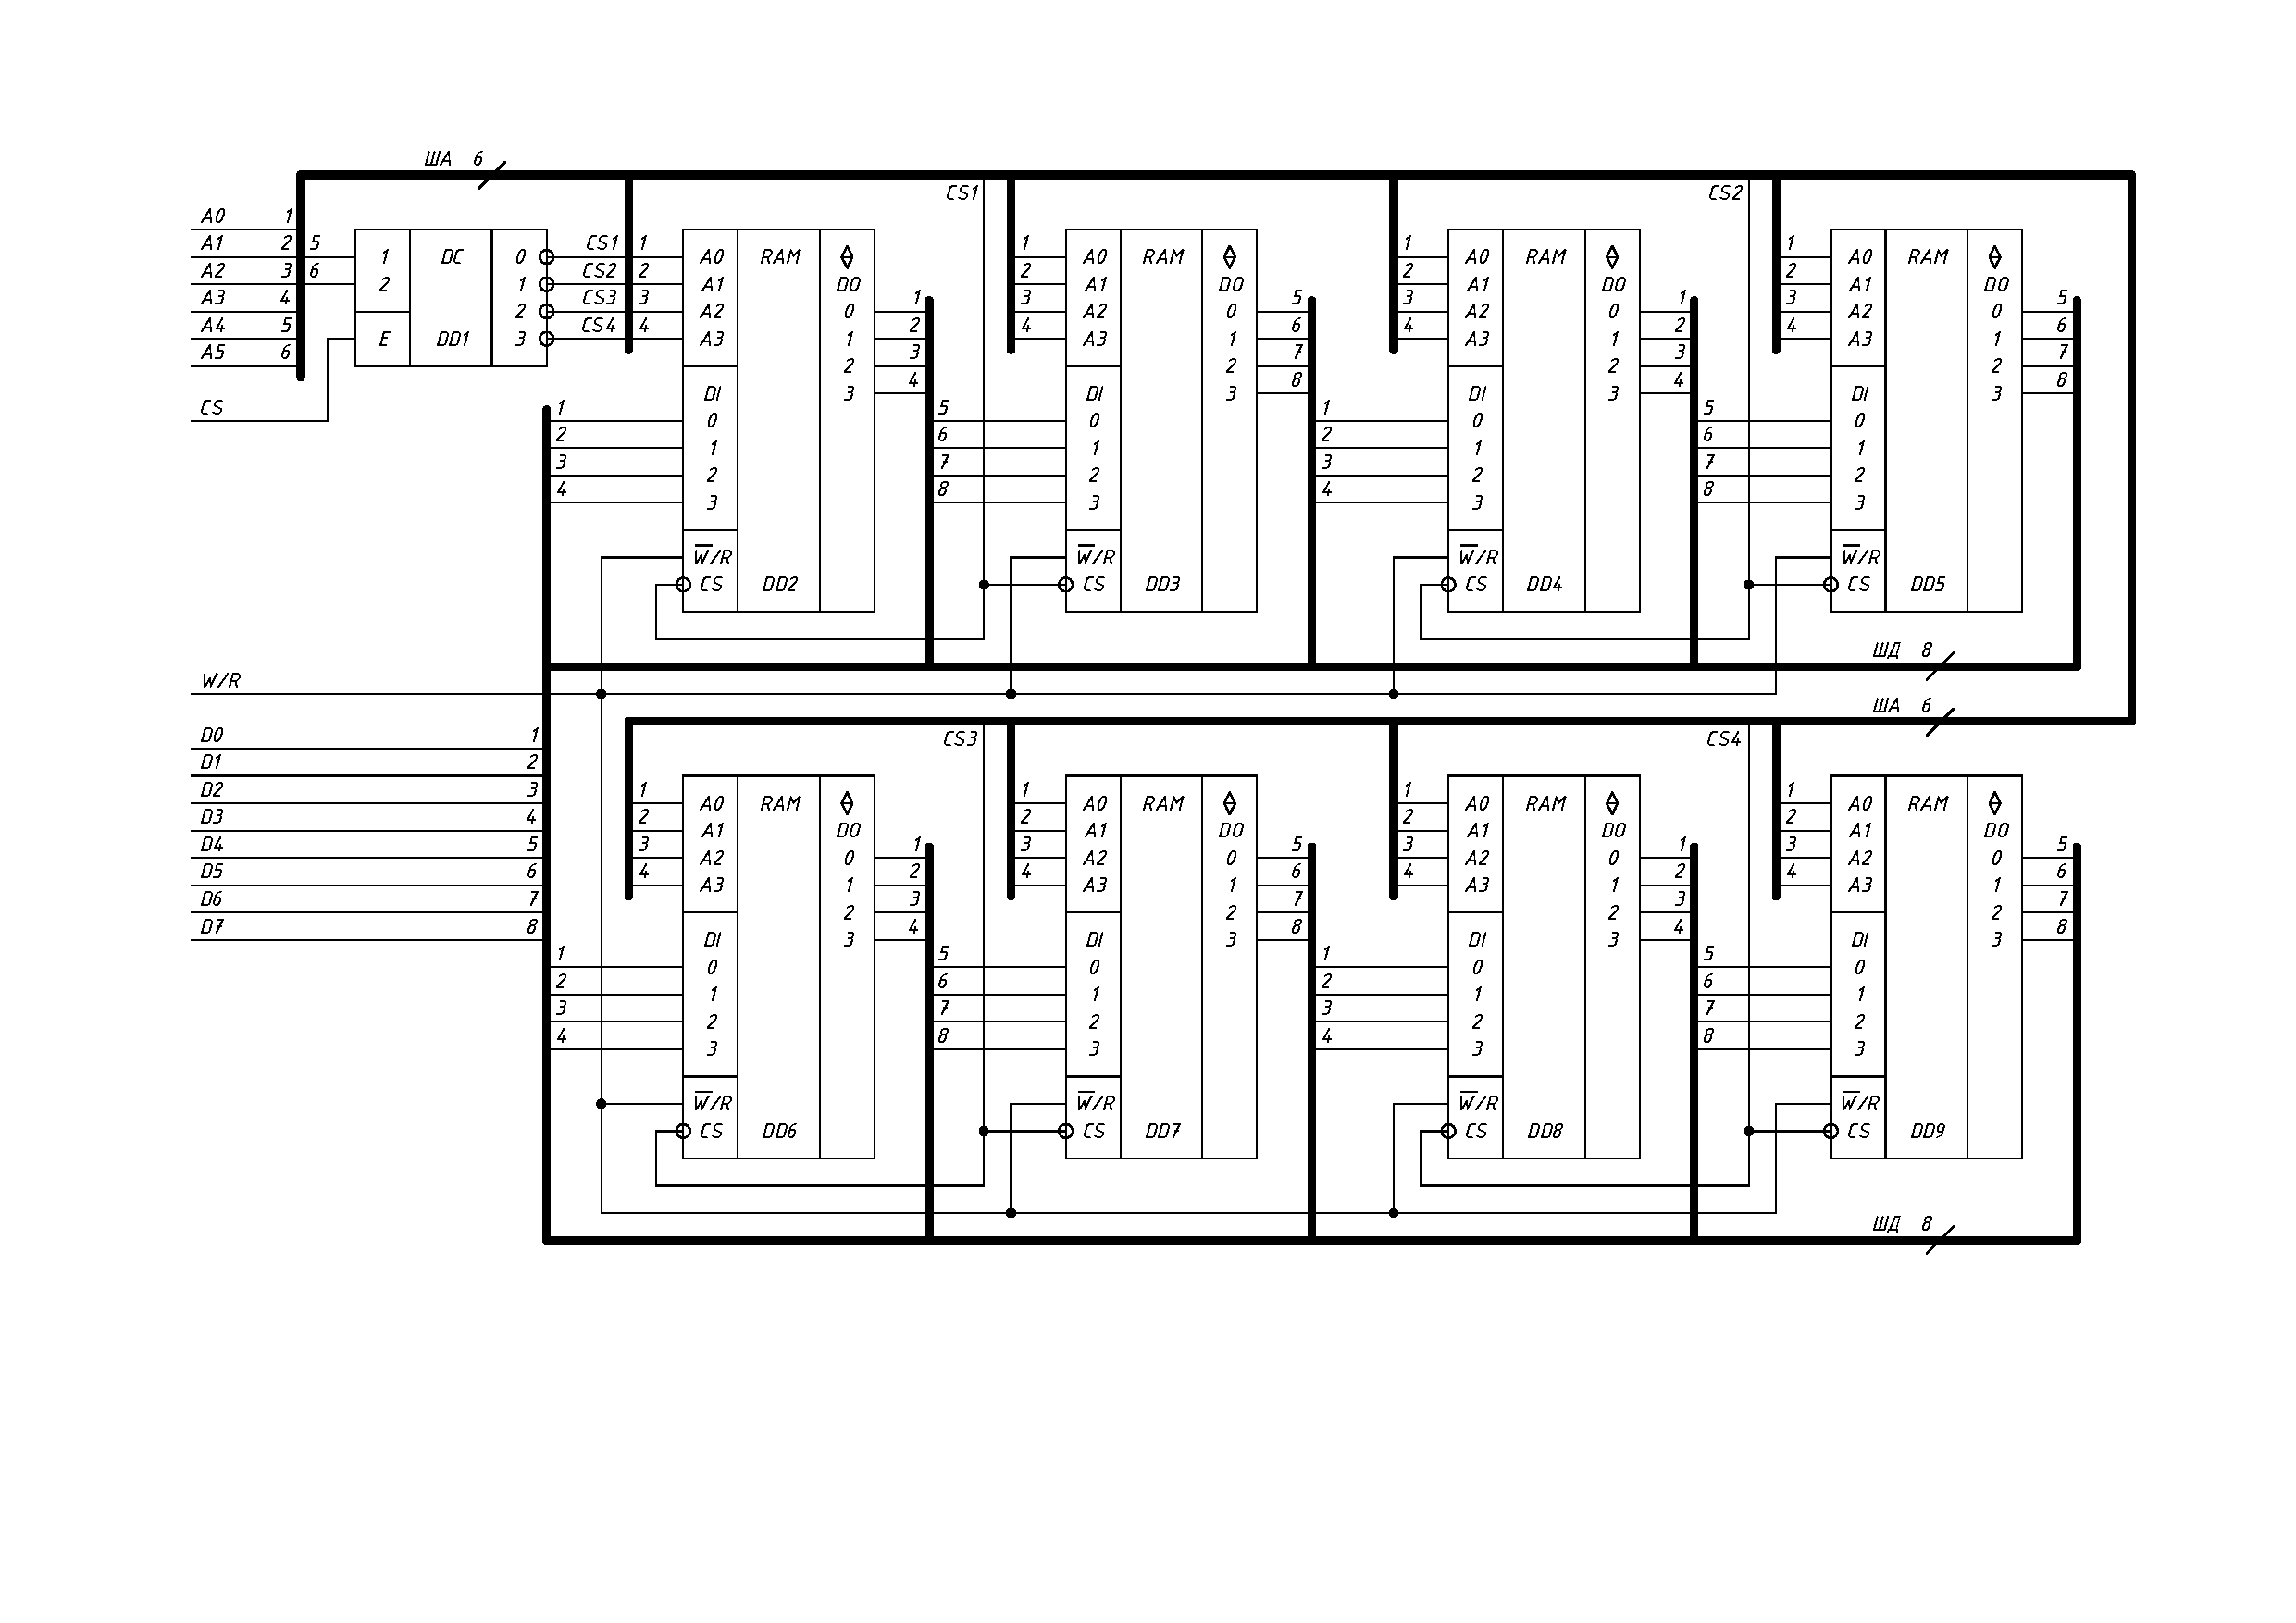
\includegraphics{img/sch4.pdf}}}}
% \end{picture}

\AddToHookNext{shipout/background}
   %{\put(0,-\paperheight){\frame{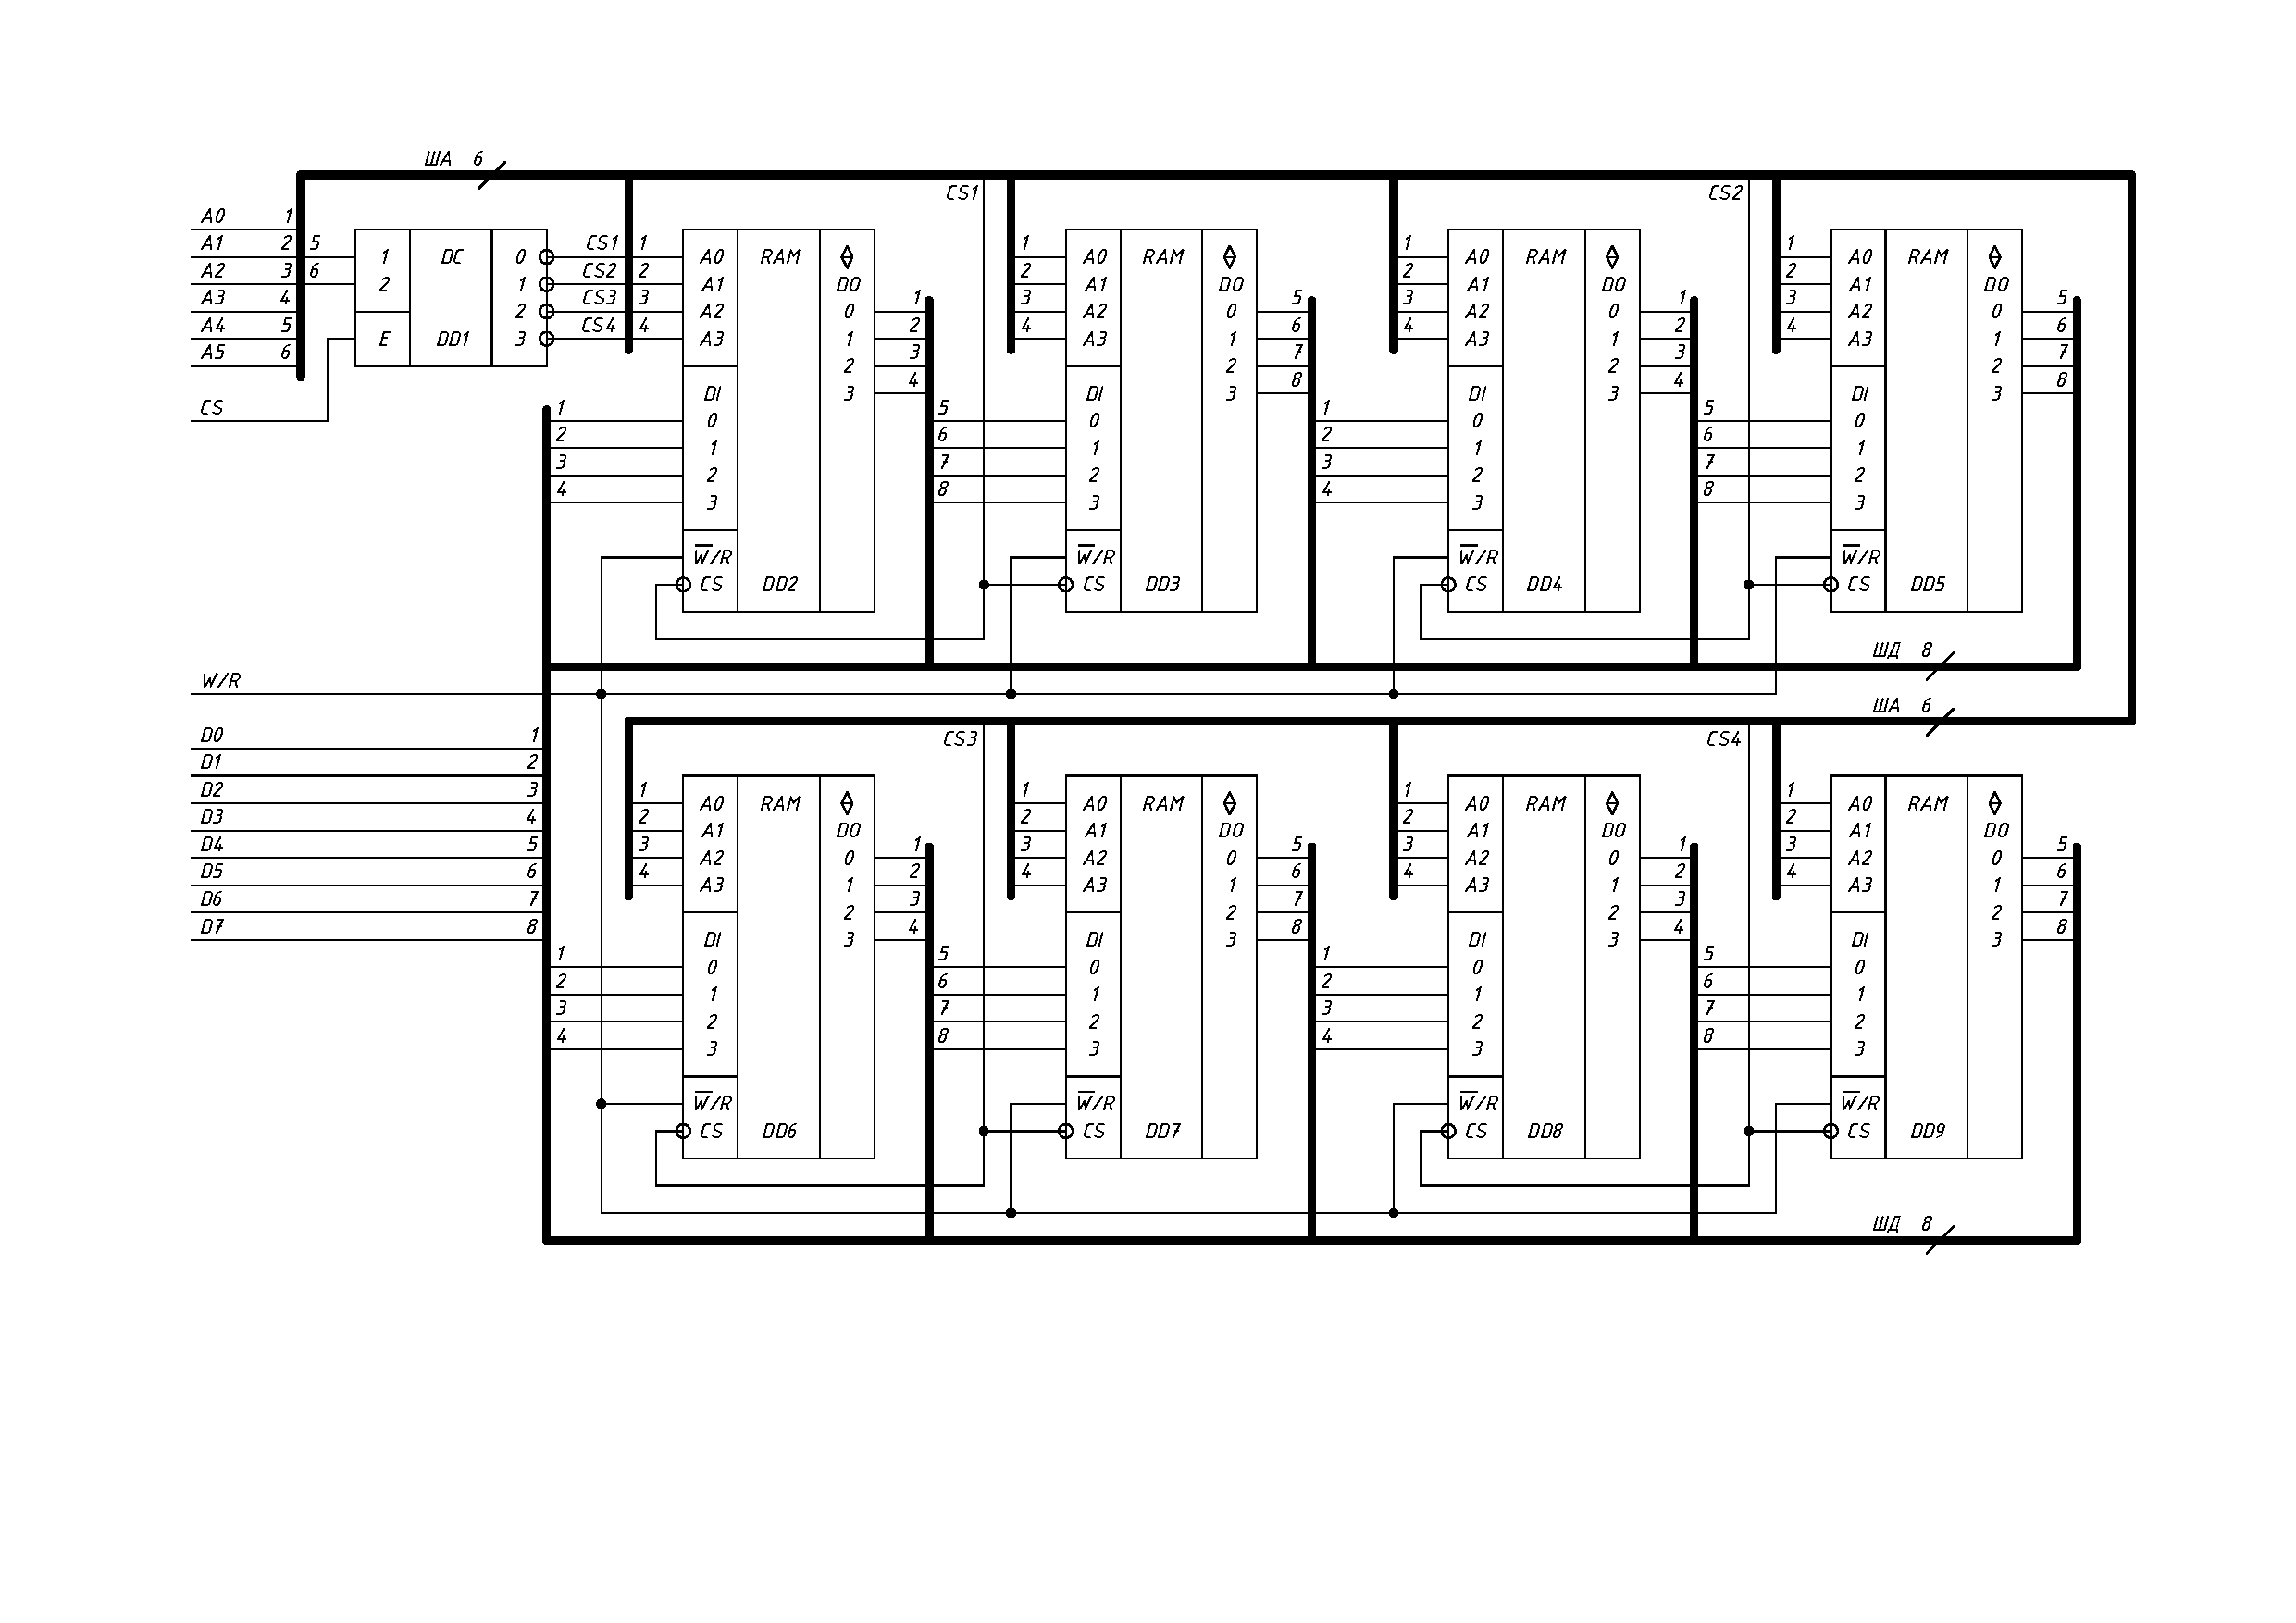
\includegraphics{img/sch4.pdf}}}}
   {\put(0,-\paperheight){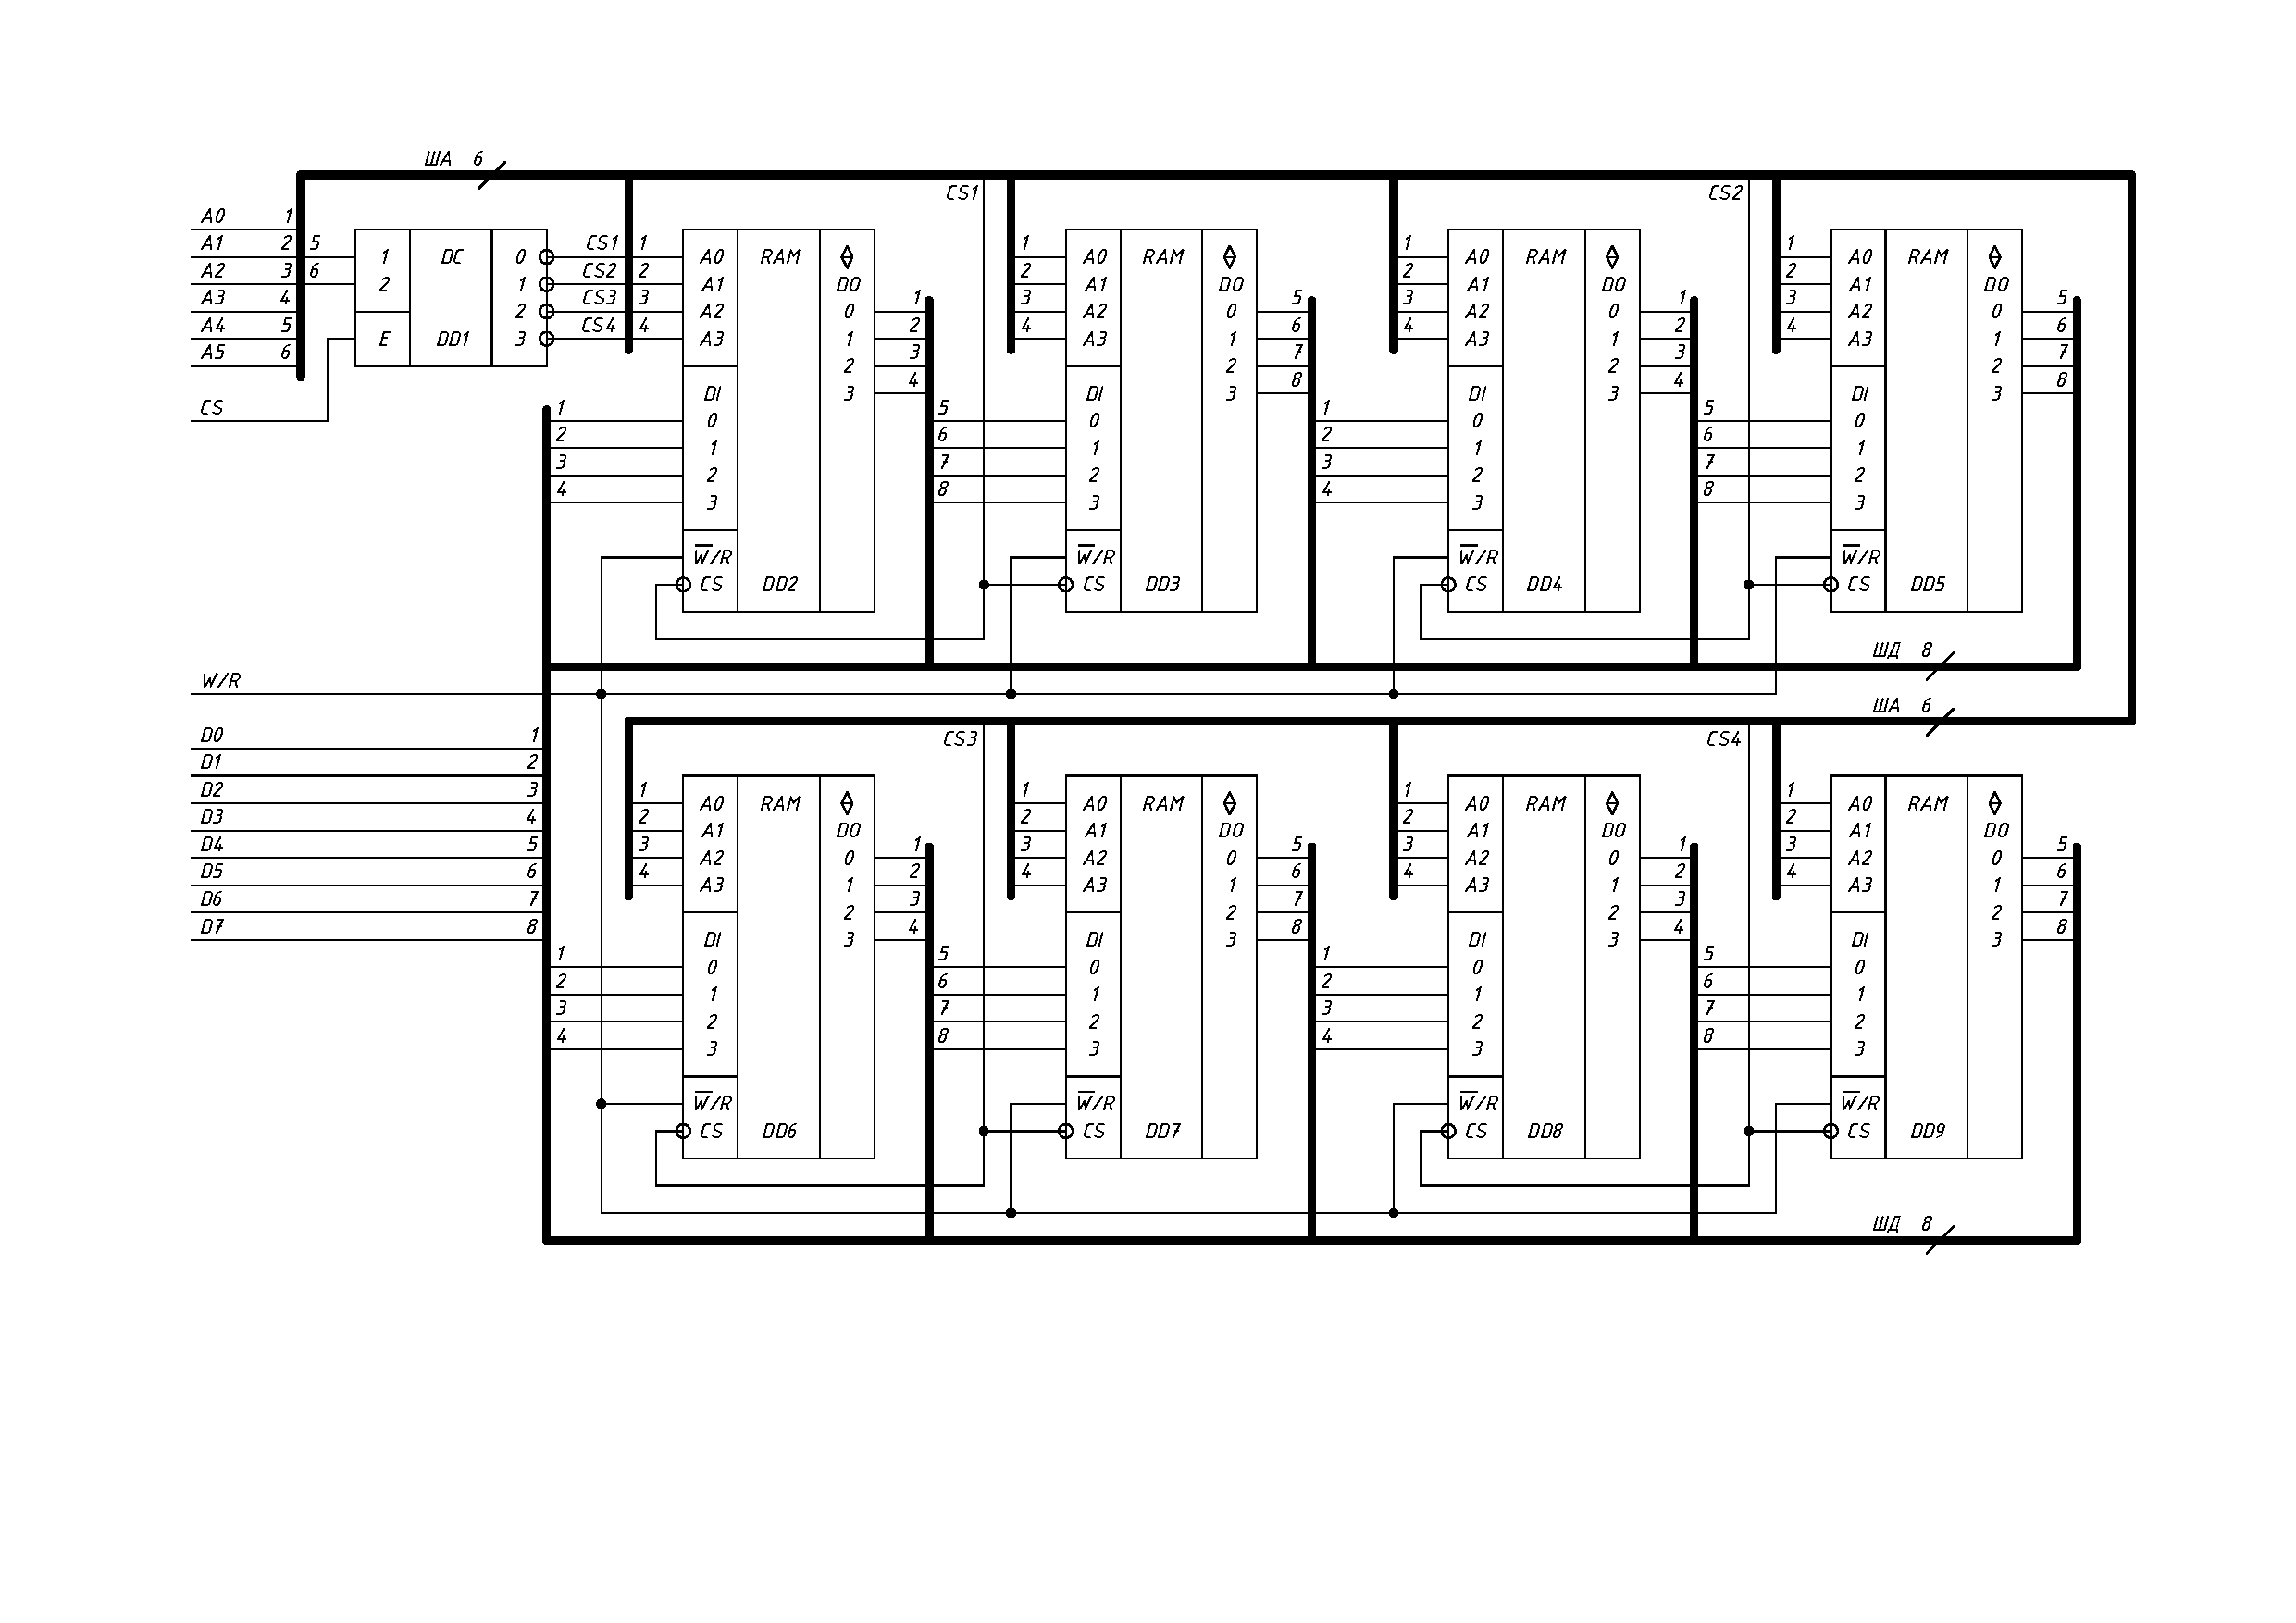
\includegraphics{img/sch4.pdf}}}
\end{drawing}
%\newgeometry{a4paper,left=3cm,top=2.0cm,bottom=2.5cm,right=1.5cm,layoutvoffset=0.5cm}

